\section{Methodology}
\label{sec:method}

Given a single RGB image, the detector estimates whether the image contains an AI-generated edit and assigns a score to each pixel. An original image is unnecessary at inference. The whole-image view supplies context, while overlapping crops retain local detail that resizing can suppress. Reference edit masks provide pixel targets during training and are used to measure localization during evaluation.

\subsection{Content and residual features}

The larger detector uses a pretrained ConvNeXt-Base~\cite{convnext} and a frozen DINOv2 ViT-Base/14~\cite{dinov2}. ConvNeXt provides features at strides 4, 8, 16, and 32. Intermediate DINOv2 features are interpolated to those same scales. At each scale, the two content representations are concatenated and projected to 128 channels. A separate forensic encoder applies 30 fixed spatial rich model filters and 30 learned constrained convolutions~\cite{bayar}. Its residual blocks provide feature maps at strides 2, 4, 8, and 16.

At stride 16, an eight-head cross-attention block uses the forensic features as queries and the corresponding content features as keys and values. A learned gate combines the attended and content features. A top-down pyramid then incorporates the stride-8 and stride-4 maps through spatial gates. The stride-2 residual features refine the mask before bilinear upsampling to the input resolution. The compact configuration uses ConvNeXt-Small and frozen DINOv2 ViT-Small/14, with gated fusion in place of cross-attention.

The image classification head pools the stride-32 content map with global average and maximum pooling. It appends the mean of the highest 2,048 mask logits, or all mask logits when fewer are available, and maps the resulting vector to one logit. This pooling occurs within a single image or crop forward pass. The full-image tile aggregation described below uses a different pooling rule.

\subsection{Training configurations}

The compact and larger checkpoints used by the ensemble were obtained with an earlier crop-based procedure. That procedure sampled $384\times384$ crops and retained each source image's classification label. An edited image could therefore contribute a crop with zero annotated edited pixels and a positive image label. The ensemble results characterize these historical checkpoints.

The later joint-view experiment addressed this supervision mismatch. For each source image, the same network processes a $384\times384$ resized whole image and a crop at the input pixel scale when the image dimensions permit it. The whole view receives the source image label. The crop receives a positive label only when its mask contains edited pixels. The crop sampler favors regions near the edit during training, and each mini-batch balances genuine and edited source images. The joint objective combines whole-image classification, crop classification, pixel segmentation, and penalties on predicted edit probabilities for genuine whole views and empty-mask crops:
\begin{equation}
  \mathcal{L}=\mathcal{L}_{\mathrm{whole}}+0.5\mathcal{L}_{\mathrm{crop}}+
  \mathcal{L}_{\mathrm{seg}}+0.3\left(\mathcal{L}_{\mathrm{bg,w}}+\mathcal{L}_{\mathrm{bg,c}}\right).
\end{equation}
Classification uses binary cross-entropy. For crops with edited pixels, segmentation uses balanced pixel binary cross-entropy and Dice loss. Checkpoint selection for this experiment uses whole-image balanced accuracy on validation.

\subsection{Inference and decisions}

\begin{figure*}[t]
\centering
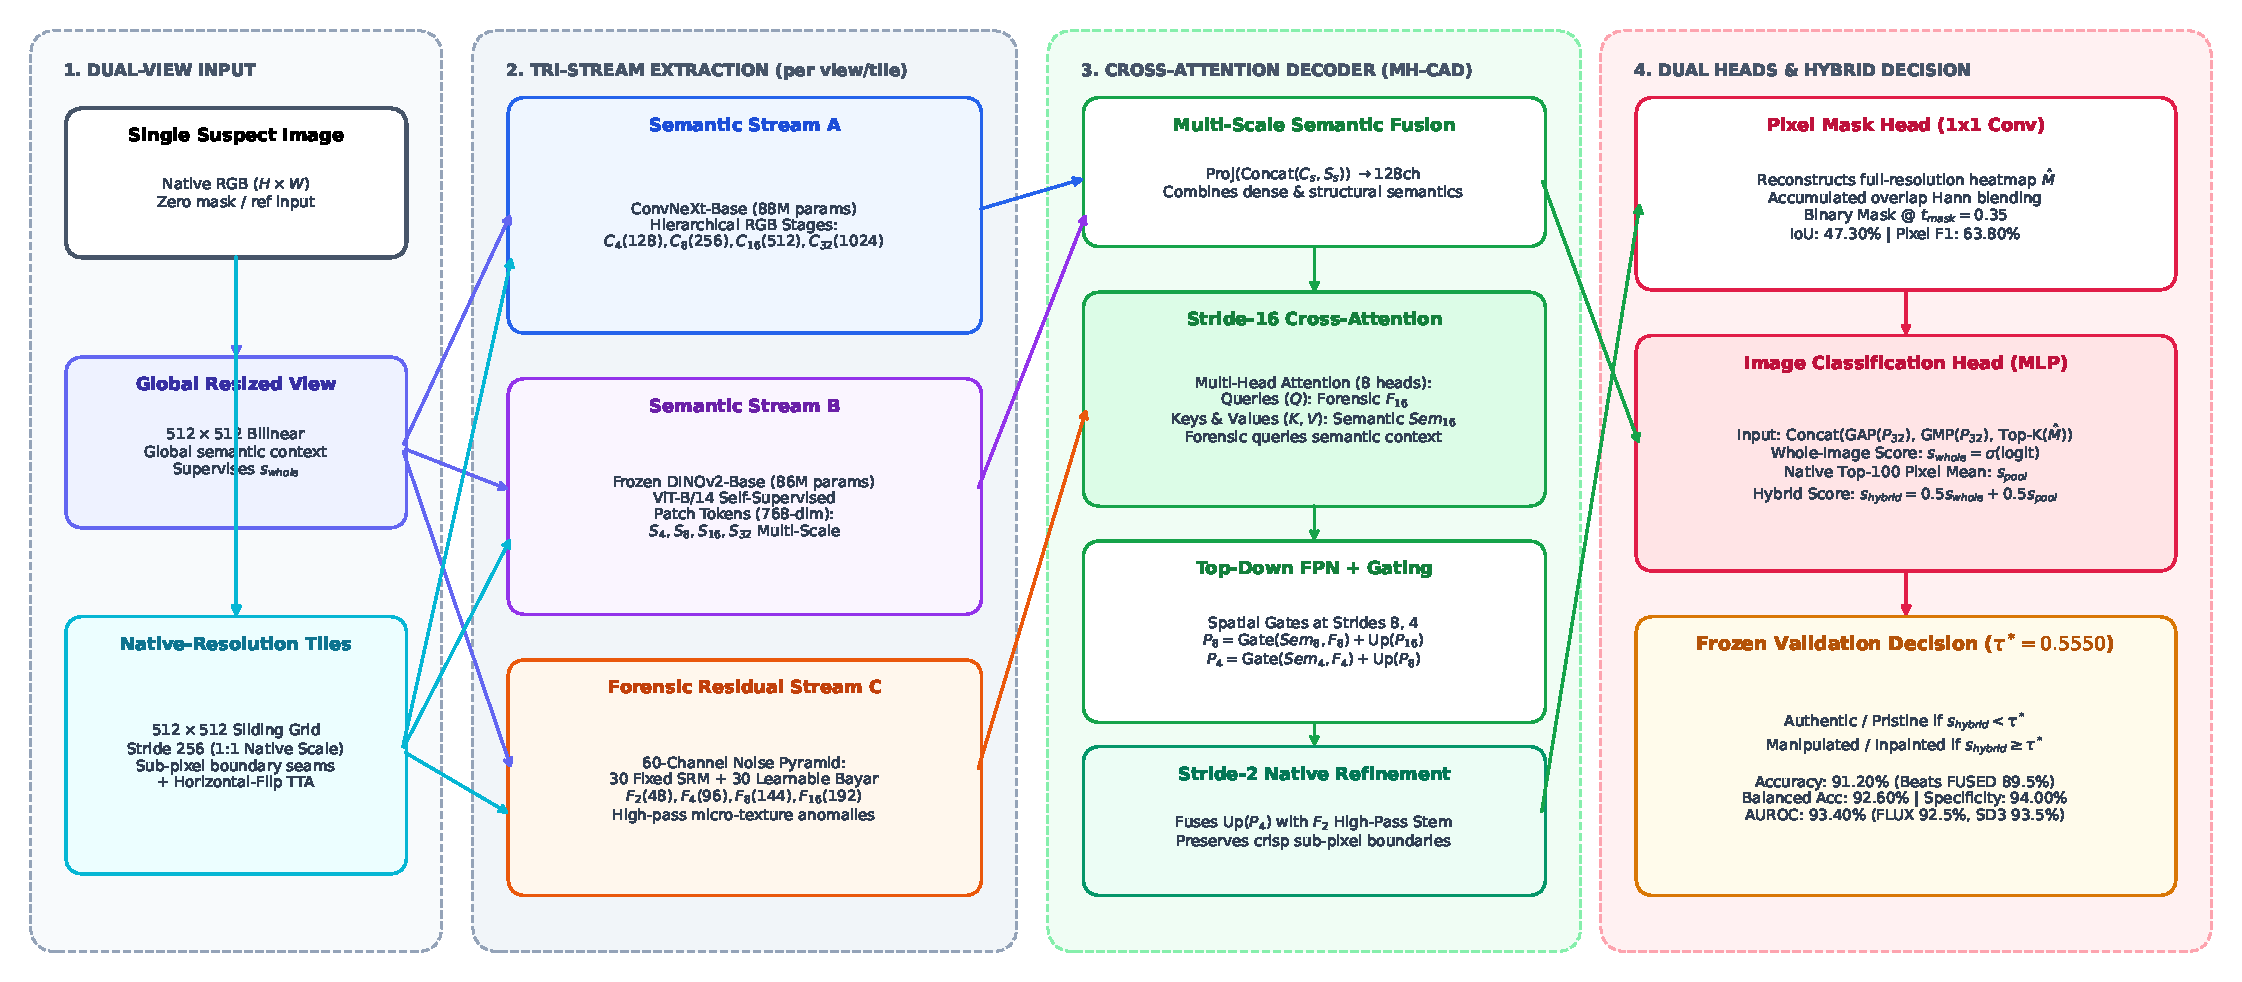
\includegraphics[width=\textwidth]{figures/architecture.pdf}
\caption{Overview of the proposed SuperFRAME v2 architecture. (1) A single unconstrained RGB image is decomposed into a resized global view for macroscopic context and sliding native-resolution tiles ($1:1$ scale) with horizontal-flip test-time augmentation (TTA) to preserve subtle inpainting seams. (2) Each view is independently encoded by a Tri-Stream feature extractor: ConvNeXt-Base (dense hierarchical semantics), frozen DINOv2-Base (self-supervised patch tokens), and a 60-channel SRM/Bayar noise residual pyramid. (3) The Multi-Head Cross-Attention Decoder (MH-CAD) fuses residual queries with semantic key/values, guided by spatial gating and Stride-2 high-pass refinement. (4) The pixel mask head outputs the continuous manipulation heatmap $\hat{M}$ (thresholded at $t_{\text{mask}}=0.35$), while the image detection head aggregates global feature pooling and top-100 tile anomaly scores into a calibrated hybrid decision ($s_{\text{hybrid}}$ at $\tau^*=0.5550$).}
\Description{SuperFRAME v2 pipeline showing dual-view input, tri-stream feature extraction, multi-head cross-attention decoder, and dual output heads for pixel localization and whole-image classification.}
\label{fig:architecture}
\end{figure*}

Figure~\ref{fig:inference} shows the two views used during ensemble inference. Whole-image scores are the weighted mean of the larger and compact models' sigmoid outputs, with weights 0.65 and 0.35. Localization runs on $384\times384$ tiles with a stride of 256 pixels. Tile logits use the same model weights and are averaged with the predictions from horizontally flipped tiles mapped back to the original orientation. Overlapping probability maps are merged with Hann weights. The mask is thresholded at 0.35, then holes are filled and connected components smaller than 64 pixels are removed.

Let $s_{\mathrm{whole}}$ denote the whole-image score and $s_{\mathrm{local}}$ the mean of the 100 highest pixel scores in the merged probability map. The ensemble image score is
\begin{equation}
  s=0.15s_{\mathrm{whole}}+0.85s_{\mathrm{local}}.
\end{equation}
The reported ensemble evaluation applies an image threshold of 0.9358 inherited from an earlier calibration. The threshold has not been independently fitted for the ensemble. The separate score audit compares whole-image, local, and combined scores and selects thresholds on validation by balanced accuracy.
